\documentclass[journal,12pt,twocolumn]{IEEEtran}
\usepackage[compact]{titlesec}
\usepackage{setspace}
\usepackage{gensymb}
\singlespacing
\usepackage[cmex10]{amsmath}
\usepackage{amsthm}
\usepackage{mathrsfs}
\usepackage{txfonts}
\usepackage{stfloats}
\usepackage{bm}
\usepackage{cite}
\usepackage{cases}
\usepackage{subfig}
\usepackage{longtable}
\usepackage{multirow}
\usepackage{enumitem}
\usepackage{mathtools}
\usepackage{steinmetz}
\usepackage{tikz}
\usepackage{circuitikz}
\usepackage{verbatim}
\usepackage{tfrupee}
\usepackage[breaklinks=true]{hyperref}
\usepackage{tkz-euclide}

\usetikzlibrary{calc,math}
\usepackage{listings}
    \usepackage{color}                                            %%
    \usepackage{array}                                            %%
    \usepackage{longtable}                                        %%
    \usepackage{calc}                                             %%
    \usepackage{multirow}                                         %%
    \usepackage{hhline}                                           %%
    \usepackage{ifthen}                                           %%

    \usepackage{lscape}     
\usepackage{multicol}
\usepackage{chngcntr}

\DeclareMathOperator*{\Res}{Res}
\renewcommand\thesection{\arabic{section}}
\renewcommand\thesubsection{\thesection.\arabic{subsection}}
\renewcommand\thesubsubsection{\thesubsection.\arabic{subsubsection}}

\renewcommand\thesectiondis{\arabic{section}}
\renewcommand\thesubsectiondis{\thesectiondis.\arabic{subsection}}
\renewcommand\thesubsubsectiondis{\thesubsectiondis.\arabic{subsubsection}}

\hyphenation{op-tical net-works semi-conduc-tor}
\def\inputGnumericTable{}                                 %%

\lstset{
frame=single, 
breaklines=true,
columns=fullflexible
}

\begin{document}

\newtheorem{theorem}{Theorem}[section]
\newtheorem{problem}{Problem}
\newtheorem{proposition}{Proposition}[section]
\newtheorem{lemma}{Lemma}[section]
\newtheorem{corollary}[theorem]{Corollary}
\newtheorem{example}{Example}[section]
\newtheorem{definition}[problem]{Definition}
\newcommand{\BEQA}{\begin{eqnarray}}
\newcommand{\EEQA}{\end{eqnarray}}
\newcommand{\define}{\stackrel{\triangle}{=}}
\bibliographystyle{IEEEtran}

\providecommand{\mbf}{\mathbf}
\providecommand{\pr}[1]{\ensuremath{\Pr\left(#1\right)}}
\providecommand{\qfunc}[1]{\ensuremath{Q\left(#1\right)}}
\providecommand{\sbrak}[1]{\ensuremath{{}\left[#1\right]}}
\providecommand{\lsbrak}[1]{\ensuremath{{}\left[#1\right.}}
\providecommand{\rsbrak}[1]{\ensuremath{{}\left.#1\right]}}
\providecommand{\brak}[1]{\ensuremath{\left(#1\right)}}
\providecommand{\lbrak}[1]{\ensuremath{\left(#1\right.}}
\providecommand{\rbrak}[1]{\ensuremath{\left.#1\right)}}
\providecommand{\cbrak}[1]{\ensuremath{\left\{#1\right\}}}
\providecommand{\lcbrak}[1]{\ensuremath{\left\{#1\right.}}
\providecommand{\rcbrak}[1]{\ensuremath{\left.#1\right\}}}
\theoremstyle{remark}
\newtheorem{rem}{Remark}
\newcommand{\sgn}{\mathop{\mathrm{sgn}}}
\providecommand{\abs}[1]{\left\vert#1\right\vert}
\providecommand{\res}[1]{\Res\displaylimits_{#1}} 
\providecommand{\norm}[1]{\left\lVert#1\right\rVert}

\providecommand{\mtx}[1]{\mathbf{#1}}
\providecommand{\mean}[1]{E\left[ #1 \right]}
\providecommand{\fourier}{\overset{\mathcal{F}}{ \rightleftharpoons}}

\providecommand{\system}{\overset{\mathcal{H}}{ \longleftrightarrow}}
\newcommand{\solution}{\noindent \textbf{Solution: }}
\newcommand{\cosec}{\,\text{cosec}\,}
\providecommand{\dec}[2]{\ensuremath{\overset{#1}{\underset{#2}{\gtrless}}}}
\newcommand{\myvec}[1]{\ensuremath{\begin{pmatrix}#1\end{pmatrix}}}
\newcommand{\mydet}[1]{\ensuremath{\begin{vmatrix}#1\end{vmatrix}}}
\numberwithin{equation}{subsection}

\makeatletter
\@addtoreset{figure}{problem}
\makeatother
\let\StandardTheFigure\thefigure
\let\vec\mathbf

\renewcommand{\thefigure}{\theproblem}

\def\putbox#1#2#3{\makebox[0in][l]{\makebox[#1][l]{}\raisebox{\baselineskip}[0in][0in]{\raisebox{#2}[0in][0in]{#3}}}}
     \def\rightbox#1{\makebox[0in][r]{#1}}
     \def\centbox#1{\makebox[0in]{#1}}
     \def\topbox#1{\raisebox{-\baselineskip}[0in][0in]{#1}}
     \def\midbox#1{\raisebox{-0.5\baselineskip}[0in][0in]{#1}}
\vspace{3cm}
\title{Assignment-6}
\author{Vipul Kumar Malik}

\date{\today}

\maketitle
\newpage
\bigskip
\renewcommand{\thefigure}{\theenumi}
\renewcommand{\thetable}{\theenumi}

\begin{abstract}
This document explains the concept of finding the equation of tangent to a circle using linear algebra.
\end{abstract}
Download all python codes from 
\begin{lstlisting}
https://github.com/vipulmalik8569/MT-EE5609
\end{lstlisting}
and latex-tikz codes from 
\begin{lstlisting}
https://github.com/vipulmalik8569/MT-EE5609
\end{lstlisting}
\section{\textbf{Problem}}
Write down the equation of the tangent to a circle passing through the point $\vec{p}$. 

Equation of the circle and positional vector $\vec{p}$ is given as :
\begin{align}
    x^2+y^2-3x+10y&=15\label{eq:0}\\
    \vec{p}&=\myvec{4\\-11}
\end{align}

\section{\textbf{Solution}}


General equation of the circle in vector form is :
\begin{align}
\vec{x}^T\vec{x}+2\vec{u}^T\vec{x}+f=0\label{eq:1}
\end{align}
In the vector form \eqref{eq:0} can be written as :
\begin{align}
\vec{x}^T\vec{x}+2\myvec{\frac{-3}{2}\\[0.1 cm]5}^T\vec{x}-15=0\label{eq:2}
\end{align}
By comparing \eqref{eq:1} and \eqref{eq:2} we get : 
\begin{align}
    \vec{u}=\myvec{-\frac{3}{2}\\[0.1 cm]5},f=-15\label{eq:3}
\end{align}
We know that the equation of tangent in the form of normal vector $(\vec{p}+\vec{u})$ and point $\vec{p}$ can be written as:
\begin{align}
    (\vec{p}+\vec{u})^T(\vec{x}-\vec{p})&=0\\
    (\vec{p}+\vec{u})^T\vec{x}-\vec{p}^T\vec{p}-\vec{u}^T\vec{q}&=0\label{eq:5}
\end{align}
Using \eqref{eq:1}, \eqref{eq:5} will become : 
\begin{align}
    (\vec{p}+\vec{u})^T\vec{x}+\vec{u}^T\vec{p}+f&=0\label{eq:6}
\end{align}
By putting the values of $\vec{p}$, $\vec{u}$ and $f$ from \eqref{eq:3} in \eqref{eq:6} we get : 
\begin{align}
    \myvec{\frac{5}{2}&-6}\vec{x}+\myvec{4&-11}\myvec{\frac{-3}{2}\\[0.2cm]5}-15&=0\\
    \myvec{\frac{5}{2}&-6}\vec{x}-76&=0
\end{align}
Hence the equation of the tangent to the circle passing through the point $\vec{p}$ is:
\begin{align}
    \myvec{\frac{5}{2}&-6}\vec{x}&=76\label{eq:9}
\end{align}
Plot of the tangent to a circle given by equation \eqref{eq:9} is as follows :
\begin{figure}[h]
\centering
    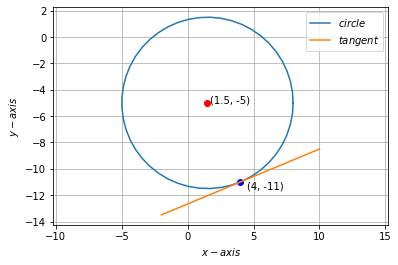
\includegraphics[width=\columnwidth]{tangent.png}
    \caption{Tangent to a circle centered at $(1.5, -5)$ with radius $6.5$ passing through the point $(4,-11)$.}
    \label{tangent}
\end{figure}
\end{document}

